\documentclass[xcolor=table]{beamer}
% generated by Madoko, version 1.0.3
%mdk-data-line={1}


\usepackage[heading-base={2},section-num={False},bib-label={True}]{madoko2}
%mdk-data-line={1;out\presentation.mdk:79}

    \ifbeamer\relax\else
      \providecommand{\usetheme}[2][]{}
      \providecommand{\usecolortheme}[2][]{}
      \providecommand{\usefonttheme}[2][]{}
      \providecommand{\pause}[1][]{}
      \providecommand{\AtBeginSection}[2][]{}
      \providecommand{\AtBeginSubsection}[2][]{}
      \providecommand{\AtBeginSubsubsection}[2][]{}
      \providecommand{\AtBeginPart}[2][]{}
      \providecommand{\AtBeginLecture}[2][]{}
      \providecommand{\theoremstyle}[2][]{}
      \makeatletter
      \def\newtheorem{\@ifstar\newtheoremx\newtheoremx}
      \makeatother
      \providecommand{\newtheoremx}[3][]{}{}
    \fi
%mdk-data-line={1;out\presentation.mdk:96}

    \ifbeamer\usetheme[]{singapore}\fi
\begin{document}



%mdk-data-line={10}
%mdk-data-line={10}
%mdk-data-line={11}
\mdxtitleblockstart{}
%mdk-data-line={11}
\mdxtitle{{\mdfontsize{3em}\mdline{11}数独浅谈}}%mdk

%mdk-data-line={14}
\mdxsubtitle{{\mdfontsize{1.8em}\mdline{14}古老的数字逻辑游戏}}%mdk
\mdxauthorstart{\Large{}
%mdk-data-line={19}
\mdxauthorname{{\mdfontsize{1.4em}\mdline{19}符晓浛}}%mdk

%mdk-data-line={22}
\mdxauthoraddress{\mdline{22}上海交通大学}%mdk

%mdk-data-line={25}
\mdxauthoremail{\mdline{25}reapor.yurnero@sjtu.edu.cn}%mdk
}\mdxauthorend\mdtitleauthorrunning{}{}\mdxtitleblockend%mdk

%mdk-data-line={13}
\begin{mdframe}%mdk

\frametitle{标准数独}\label{heading-section}%mdk%mdk

%mdk-data-line={15}
\begin{mdcenter}%mdk

%mdk-data-line={16}
\noindent\mdline{16}\includegraphics[keepaspectratio=true,height=\dimpx{350}]{https:/upload.wikimedia.org/wikipedia/commons/thumb/f/ff/Sudoku-by-L2G-20050714.svg/364px-Sudoku-by-L2G-20050714.svg}{}%mdk
%mdk
\end{mdcenter}%mdk

%mdk-data-line={19}
\mdhr{}%mdk

%mdk-data-line={20}
\noindent\mdline{20}数独 (日语:数独/すうどく Sūdoku)是一种逻辑性的数字填充游戏,玩家须以数字填进每一格,而每行、每列和每个宫(即3x3的大格)有齐1至9所有数字。游戏设计者会提供一部分的数字,使谜题只有一个答案。%mdk
%mdk
\end{mdframe}\label{section}%mdk%mdk

%mdk-data-line={24}
\begin{mdframe}%mdk

\frametitle{数独的历史}\label{heading-section}%mdk%mdk

%mdk-data-line={26}
\noindent\mdline{26}数独起源于18世纪初瑞士数学家欧拉等人研究的拉丁方阵(Latin Square)。
19世纪80年代,一位美国的退休建筑师格昂斯(Howard Garns)根据这种拉丁方阵发明了一种填数趣味游戏,这就是数独的雏形。20世纪70年代,人们在美国纽约的一本益智杂志《Math Puzzles and Logic Problems》上发现了这个游戏,当时被称为填数字(Number Place),这也是目前公认的数独最早的见报版本。1984年一位日本学者将其介绍到了日本,发表在Nikoli公司的一本游戏杂志上,当时起名为“Suuji wa dokushin ni kagiru”,就改名为“sudoku”,其中“su”是数字的意思,“doku”是单一的意思。后来一位前任香港高等法院的新西兰籍法官高乐德(Wayne Gould)在1997年3月到日本东京旅游时,无意中发现了。
他首先在英国的《泰晤士报》上发表,不久其他报纸也发表,很快便风靡全英国。随着计算机信息技术的发展,数独开始在全世界流行。%mdk
%mdk
\end{mdframe}\label{section}%mdk%mdk

%mdk-data-line={30}
\begin{mdframe}%mdk

\frametitle{规则}\label{heading-section}%mdk%mdk

%mdk-data-line={32}
\noindent\mdline{32}数独的规则非常简单:%mdk

%mdk-data-line={34}
\begin{itemize}[noitemsep,topsep=\mdcompacttopsep]%mdk

%mdk-data-line={34}
\item\mdline{34}每一行由1\mdline{34}\textasciitilde{}\mdline{34}9单独出现一次%mdk

%mdk-data-line={35}
\item\mdline{35}每一列由1\mdline{35}\textasciitilde{}\mdline{35}9单独出现一次%mdk

%mdk-data-line={36}
\item\mdline{36}每一个小的九宫格1\mdline{36}\textasciitilde{}\mdline{36}9由单独出现一次%mdk
%mdk
\end{itemize}%mdk
%mdk
\end{mdframe}\label{section}%mdk%mdk

%mdk-data-line={40}
\begin{mdframe}%mdk

\frametitle{解谜技巧}\label{heading-section}%mdk%mdk

%mdk-data-line={41}
\noindent\mdline{41}由上述的三条基本规则,我们可以衍生出摸索出一些简单实用的技巧。学习这些技巧,能有效的缩短解题的时间。\mdline{41}%mdk

%mdk-data-line={43}
\mdline{43}不过大家要始终牢记,所有的方法都来源于规则,因此,没有必要拘泥于一些所谓的方法,这些方法只是一些辅助,深入理解规则才是王道。%mdk

%mdk-data-line={45}
\begin{mdcenter}%mdk

%mdk-data-line={46}
\noindent\mdline{46}\includegraphics[keepaspectratio=true]{https:/upload.wikimedia.org/wikipedia/commons/thumb/f/ff/Sudoku-by-L2G-20050714.svg/364px-Sudoku-by-L2G-20050714.svg}{}%mdk
%mdk
\end{mdcenter}%mdk
%mdk
\end{mdframe}\label{section}%mdk%mdk

%mdk-data-line={49}
\begin{mdframe}%mdk

\frametitle{查找空缺法}\label{heading-section}%mdk%mdk

%mdk-data-line={50}
\begin{mdcenter}%mdk

%mdk-data-line={51}
\noindent\mdline{51}   此方法常用于即将完成(已知6、7、8个数)的行、列、宫。%mdk
%mdk
\end{mdcenter}%mdk
\begin{mdtabular}{2}{\dimeval{(\linewidth-\dimwidth{0.50})/1}}{0pt}%mdk
\begin{tabular}{ll}

%mdk-data-line={55}
\begin{mdcolumn}%mdk
\begin{mdblock}{width=\dimwidth{0.50}}%mdk
%mdk-data-line={56}
\noindent\mdline{56}\includegraphics[keepaspectratio=true,width=\dimpx{480}]{http:/www.conceptispuzzles.com/zh/picture/27/1194}{}\mdline{56}%mdk%mdk
\end{mdblock}%mdk
\end{mdcolumn}%mdk
&
%mdk-data-line={59}
\begin{mdcolumn}%mdk
\begin{mdblock}{width=\dimavailable}%mdk
%mdk-data-line={60}
\noindent\mdline{60}  \mdline{60}\mdline{60}%mdk%mdk
\end{mdblock}%mdk
\end{mdcolumn}%mdk
\\
\end{tabular}\end{mdtabular}
%mdk
\end{mdframe}\label{section}%mdk%mdk

%mdk-data-line={65}
\begin{mdframe}%mdk

\frametitle{单向扫看法}\label{heading-section}%mdk%mdk

%mdk-data-line={66}
\begin{mdcenter}%mdk

%mdk-data-line={67}
\noindent\mdline{67}如下图所示,我们可以利用这种方法迅速地找出一些数字的正确位置。%mdk
%mdk
\end{mdcenter}%mdk
\begin{mdtabular}{2}{\dimeval{(\linewidth-\dimwidth{0.50})/1}}{0pt}%mdk
\begin{tabular}{ll}

%mdk-data-line={70}
\begin{mdcolumn}%mdk
\begin{mdblock}{width=\dimwidth{0.50}}%mdk
%mdk-data-line={71}
\noindent\mdline{71}\includegraphics[keepaspectratio=true,width=\dimpx{480}]{http:/www.conceptispuzzles.com/zh/picture/27/1186}{}\mdline{71}%mdk%mdk
\end{mdblock}%mdk
\end{mdcolumn}%mdk
&
%mdk-data-line={74}
\begin{mdcolumn}%mdk
\begin{mdblock}{width=\dimavailable}%mdk
%mdk-data-line={75}
\noindent\mdline{75}  \mdline{75}\mdline{75}%mdk%mdk
\end{mdblock}%mdk
\end{mdcolumn}%mdk
\\
\end{tabular}\end{mdtabular}
%mdk
\end{mdframe}\label{section}%mdk%mdk

%mdk-data-line={80}
\begin{mdframe}%mdk

\frametitle{双向扫看法}\label{heading-section}%mdk%mdk

%mdk-data-line={81}
\begin{mdcenter}%mdk

%mdk-data-line={82}
\noindent\mdline{82}如下图所示,这种方法是单向法的变形。这两者是最常用的方法。%mdk
%mdk
\end{mdcenter}%mdk
\begin{mdtabular}{2}{\dimeval{(\linewidth-\dimwidth{0.50})/1}}{0pt}%mdk
\begin{tabular}{ll}

%mdk-data-line={85}
\begin{mdcolumn}%mdk
\begin{mdblock}{width=\dimwidth{0.50}}%mdk
%mdk-data-line={86}
\noindent\mdline{86}\includegraphics[keepaspectratio=true,width=\dimpx{480}]{http:/www.conceptispuzzles.com/zh/picture/27/1188}{}\mdline{86}%mdk%mdk
\end{mdblock}%mdk
\end{mdcolumn}%mdk
&
%mdk-data-line={89}
\begin{mdcolumn}%mdk
\begin{mdblock}{width=\dimavailable}%mdk
%mdk-data-line={90}
\noindent\mdline{90}  \mdline{90}%mdk%mdk
\end{mdblock}%mdk
\end{mdcolumn}%mdk
\\
\end{tabular}\end{mdtabular}
%mdk
\end{mdframe}\label{section}%mdk%mdk

%mdk-data-line={94}
\begin{mdframe}%mdk

\frametitle{寻找候选法}\label{heading-section}%mdk%mdk

%mdk-data-line={95}
\begin{mdcenter}%mdk

%mdk-data-line={96}
\noindent\mdline{96}这是一种稍进阶的方法,常用来打破僵局。%mdk
%mdk
\end{mdcenter}%mdk
\begin{mdtabular}{2}{\dimeval{(\linewidth-\dimwidth{0.50})/1}}{0pt}%mdk
\begin{tabular}{ll}

%mdk-data-line={99}
\begin{mdcolumn}%mdk
\begin{mdblock}{width=\dimwidth{0.50}}%mdk
%mdk-data-line={100}
\noindent\mdline{100}\includegraphics[keepaspectratio=true,width=\dimpx{480}]{http:/www.conceptispuzzles.com/zh/picture/27/1190}{}\mdline{100}%mdk%mdk
\end{mdblock}%mdk
\end{mdcolumn}%mdk
&
%mdk-data-line={103}
\begin{mdcolumn}%mdk
\begin{mdblock}{width=\dimavailable}%mdk
%mdk-data-line={104}
\noindent\mdline{104}  \mdline{104}\mdline{104}%mdk%mdk
\end{mdblock}%mdk
\end{mdcolumn}%mdk
\\
\end{tabular}\end{mdtabular}
%mdk
\end{mdframe}\label{section}%mdk%mdk

%mdk-data-line={109}
\begin{mdframe}%mdk

\frametitle{数字排除法}\label{heading-section}%mdk%mdk

%mdk-data-line={110}
\begin{mdcenter}%mdk

%mdk-data-line={111}
\noindent\mdline{111}这是一种更进阶的方法,当你无路可走时,不妨采用此方法做一尝试。%mdk
%mdk
\end{mdcenter}%mdk
\begin{mdtabular}{2}{\dimeval{(\linewidth-\dimwidth{0.50})/1}}{0pt}%mdk
\begin{tabular}{ll}

%mdk-data-line={114}
\begin{mdcolumn}%mdk
\begin{mdblock}{width=\dimwidth{0.50}}%mdk
%mdk-data-line={115}
\noindent\mdline{115}\includegraphics[keepaspectratio=true,width=\dimpx{480}]{http:/www.conceptispuzzles.com/zh/picture/27/1192}{}\mdline{115}%mdk%mdk
\end{mdblock}%mdk
\end{mdcolumn}%mdk
&
%mdk-data-line={118}
\begin{mdcolumn}%mdk
\begin{mdblock}{width=\dimavailable}%mdk
%mdk-data-line={119}
\noindent\mdline{119}  \mdline{119}%mdk%mdk
\end{mdblock}%mdk
\end{mdcolumn}%mdk
\\
\end{tabular}\end{mdtabular}

%mdk
\end{mdframe}\label{section}%mdk%mdk

%mdk-data-line={161}
\noindent\mdline{161} \mdline{161}%mdk

%mdk-data-line={161}
\begin{mdframe}%mdk

\frametitle{实战时间}\label{heading-section}%mdk%mdk

%mdk-data-line={163}
\begin{mdcenter}%mdk

%mdk-data-line={164}
\noindent\mdline{164}下面是一道难度较低的题目,最快完成正确作答的同学,将获取精美礼品一份,前十名完成的同学,也都会获得奖品。%mdk

%mdk-data-line={165}
\mdhr{}%mdk

%mdk-data-line={166}
\noindent\mdline{166}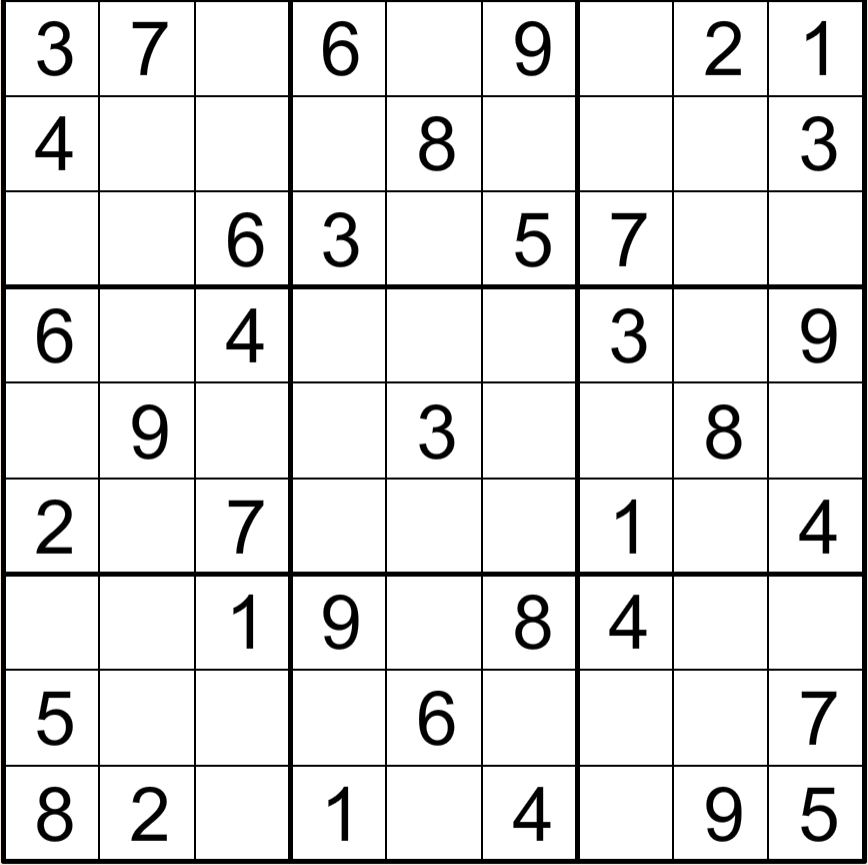
\includegraphics[keepaspectratio=true,height=\dimpx{450}]{images/sample2.1}{}\mdline{166}%mdk

%mdk-data-line={167}
\mdhr{}%mdk
%mdk
\end{mdcenter}%mdk
%mdk
\end{mdframe}\label{section}%mdk%mdk

%mdk-data-line={169}
\begin{mdframe}%mdk

\frametitle{答案揭晓}\label{heading-section}%mdk%mdk

%mdk-data-line={170}
\begin{mdcenter}%mdk

%mdk-data-line={171}
\mdhr{}%mdk

%mdk-data-line={172}
\noindent\mdline{172}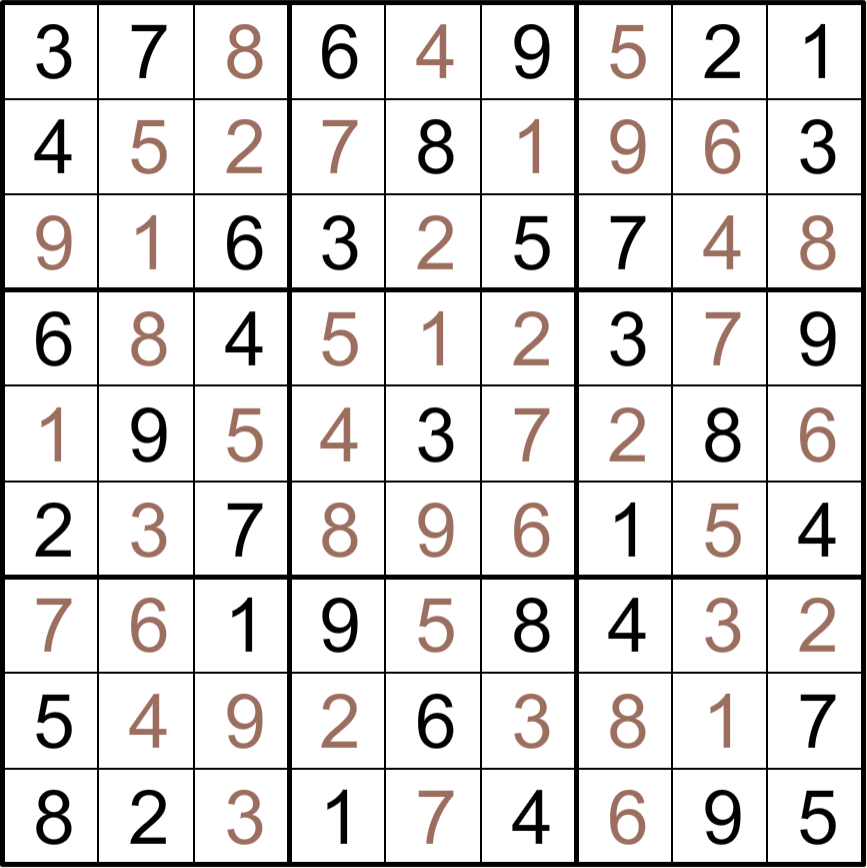
\includegraphics[keepaspectratio=true,height=\dimpx{450}]{images/sample2.2}{}\mdline{172}%mdk

%mdk-data-line={173}
\mdhr{}%mdk
%mdk
\end{mdcenter}%mdk
%mdk
\end{mdframe}\label{section}%mdk%mdk

%mdk-data-line={183}
\noindent\mdline{183} \mdline{183}%mdk

%mdk-data-line={183}
\begin{mdframe}%mdk

\frametitle{实战时间}\label{heading-section}%mdk%mdk

%mdk-data-line={185}
\begin{mdcenter}%mdk

%mdk-data-line={186}
\noindent\mdline{186}此题难度较大,大家完成第一题后可以略作尝试,能在课上完成的同学将获赠一本数独书。%mdk

%mdk-data-line={187}
\mdhr{}%mdk

%mdk-data-line={188}
\noindent\mdline{188}\includegraphics[keepaspectratio=true,height=\dimpx{450}]{https:/upload.wikimedia.org/wikipedia/commons/thumb/f/ff/Sudoku-by-L2G-20050714.svg/364px-Sudoku-by-L2G-20050714.svg}{}\mdline{188}%mdk

%mdk-data-line={189}
\mdhr{}%mdk
%mdk
\end{mdcenter}%mdk
%mdk
\end{mdframe}\label{section}%mdk%mdk

%mdk-data-line={191}
\begin{mdframe}%mdk

\frametitle{答案揭晓}\label{heading-section}%mdk%mdk

%mdk-data-line={192}
\begin{mdcenter}%mdk

%mdk-data-line={193}
\mdhr{}%mdk

%mdk-data-line={194}
\noindent\mdline{194}\includegraphics[keepaspectratio=true,height=\dimpx{450}]{https:/upload.wikimedia.org/wikipedia/commons/thumb/3/31/Sudoku-by-L2G-20050714_solution.svg/364px-Sudoku-by-L2G-20050714_solution.svg}{}\mdline{194}%mdk

%mdk-data-line={195}
\mdhr{}%mdk
%mdk
\end{mdcenter}%mdk
%mdk
\end{mdframe}\label{section}%mdk%mdk

%mdk-data-line={200}
\begin{mdframe}%mdk

\frametitle{特种数独}\label{heading-section}%mdk%mdk

%mdk-data-line={201}
\noindent\mdline{201}在标准数独之外,还有一些后来者发明的更有趣更复杂的数独,例如杀手数独、对角线数独等,我将在此为大家略作分享。%mdk

%mdk-data-line={203}
\mdline{203}但无论千变万化,数独的基本规则始终不变,只是在此基础上有所补充。%mdk
%mdk
\end{mdframe}\label{section}%mdk%mdk

%mdk-data-line={207}
\begin{mdframe}%mdk

\frametitle{变形数独}\label{heading-section}%mdk%mdk

%mdk-data-line={208}
\begin{mdcenter}%mdk

%mdk-data-line={209}
\noindent\mdline{209}原先9x9中的小九宫格变成了不规则的形状,规则也随之改变。%mdk
%mdk
\end{mdcenter}%mdk
\begin{mdtabular}{2}{\dimeval{(\linewidth-\dimwidth{0.50})/1}}{0pt}%mdk
\begin{tabular}{ll}

%mdk-data-line={213}
\begin{mdcolumn}%mdk
\begin{mdblock}{width=\dimwidth{0.50}}%mdk
%mdk-data-line={214}
\noindent\mdline{214}\includegraphics[keepaspectratio=true,width=\dimpx{450}]{https:/upload.wikimedia.org/wikipedia/commons/thumb/5/59/A_nonomino_sudoku.svg/460px-A_nonomino_sudoku.svg}{}\mdline{214}%mdk%mdk
\end{mdblock}%mdk
\end{mdcolumn}%mdk
&
%mdk-data-line={217}
\begin{mdcolumn}%mdk
\begin{mdblock}{width=\dimavailable}%mdk
%mdk-data-line={218}
\noindent\mdline{218} \mdline{218} \mdline{218}\includegraphics[keepaspectratio=true,width=\dimpx{450}]{https:/upload.wikimedia.org/wikipedia/commons/thumb/3/38/A_nonomino_sudoku_solution.svg/460px-A_nonomino_sudoku_solution.svg}{}\mdline{218}%mdk%mdk
\end{mdblock}%mdk
\end{mdcolumn}%mdk
\\
\end{tabular}\end{mdtabular}
%mdk
\end{mdframe}\label{section}%mdk%mdk

%mdk-data-line={223}
\begin{mdframe}%mdk

\frametitle{对角线数独}\label{heading-section}%mdk%mdk

%mdk-data-line={224}
\begin{mdcenter}%mdk

%mdk-data-line={225}
\noindent\mdline{225}对角线数独在标准数独的基础上,增加了主对角线也要有1\mdline{225}\textasciitilde{}\mdline{225}9单次出现的要求,难度上升。%mdk

%mdk-data-line={227}
\mdline{227}\includegraphics[keepaspectratio=true,width=\dimpx{500}]{https:/imgsa.baidu.com/baike/w/%253D268/sign=414ddf96cd95d143da76e3254bf28296/f9198618367adab4490728d68ed4b31c8601e44b
}{}%mdk
%mdk
\end{mdcenter}%mdk
%mdk
\end{mdframe}\label{section}%mdk%mdk

%mdk-data-line={230}
\begin{mdframe}%mdk

\frametitle{杀手数独}\label{heading-section}%mdk%mdk

%mdk-data-line={232}
\noindent\mdline{232}最经典的特种数独之一,在标准数独的规则基础之上,还规定了指定形状区域内的数字之和,难度较大。%mdk
\begin{mdtabular}{2}{\dimeval{(\linewidth-\dimwidth{0.50})/1}}{0pt}%mdk
\begin{tabular}{ll}

%mdk-data-line={235}
\begin{mdcolumn}%mdk
\begin{mdblock}{width=\dimwidth{0.50}}%mdk
%mdk-data-line={236}
\noindent\mdline{236}\includegraphics[keepaspectratio=true,width=\dimpx{480}]{https:/upload.wikimedia.org/wikipedia/commons/thumb/5/5e/Killersudoku_color.svg/408px-Killersudoku_color.svg}{}\mdline{236}%mdk%mdk
\end{mdblock}%mdk
\end{mdcolumn}%mdk
&
%mdk-data-line={239}
\begin{mdcolumn}%mdk
\begin{mdblock}{width=\dimavailable}%mdk
%mdk-data-line={240}
\noindent\mdline{240}\includegraphics[keepaspectratio=true,width=\dimpx{480}]{https:/upload.wikimedia.org/wikipedia/commons/thumb/8/81/Killersudoku_color_solution.svg/408px-Killersudoku_color_solution.svg}{}\mdline{240}%mdk%mdk
\end{mdblock}%mdk
\end{mdcolumn}%mdk
\\
\end{tabular}\end{mdtabular}
%mdk
\end{mdframe}\label{section}%mdk%mdk

%mdk-data-line={245}
\begin{mdframe}%mdk

\frametitle{超数独}\label{heading-section}%mdk%mdk

%mdk-data-line={246}
\begin{mdcenter}%mdk

%mdk-data-line={247}
\noindent\mdline{247}可能是最受欢迎的特种数独,难度很大。在标准数独的基础上,要求额外的九宫格满足条件。%mdk
%mdk
\end{mdcenter}%mdk
\begin{mdtabular}{2}{\dimeval{(\linewidth-\dimwidth{0.50})/1}}{0pt}%mdk
\begin{tabular}{ll}

%mdk-data-line={251}
\begin{mdcolumn}%mdk
\begin{mdblock}{width=\dimwidth{0.50}}%mdk
%mdk-data-line={252}
\noindent\mdline{252}\includegraphics[keepaspectratio=true,width=\dimpx{480}]{https:/upload.wikimedia.org/wikipedia/commons/thumb/1/12/Oceans_Hypersudoku18_Puzzle.svg/225px-Oceans_Hypersudoku18_Puzzle.svg}{}\mdline{252}%mdk%mdk
\end{mdblock}%mdk
\end{mdcolumn}%mdk
&
%mdk-data-line={255}
\begin{mdcolumn}%mdk
\begin{mdblock}{width=\dimavailable}%mdk
%mdk-data-line={256}
\noindent\mdline{256}\includegraphics[keepaspectratio=true,width=\dimpx{480}]{https:/upload.wikimedia.org/wikipedia/commons/thumb/1/17/Oceans_Hypersudoku18_Solution.svg/1000px-Oceans_Hypersudoku18_Solution.svg}{}\mdline{256}%mdk%mdk
\end{mdblock}%mdk
\end{mdcolumn}%mdk
\\
\end{tabular}\end{mdtabular}
%mdk
\end{mdframe}\label{section}%mdk%mdk

%mdk-data-line={263}
\begin{mdframe}%mdk

\frametitle{感谢您的聆听!}\label{heading-section}%mdk%mdk

%mdk
\end{mdframe}\label{section}%mdk%mdk%mdk%mdk%mdk


\end{document}
